\documentclass{article}

\usepackage{tikz}
\usetikzlibrary{calc,angles,positioning,intersections,quotes,decorations.markings,backgrounds,patterns}

\usepackage{pgfplots}
\pgfplotsset{compat=1.14}



\begin{document}

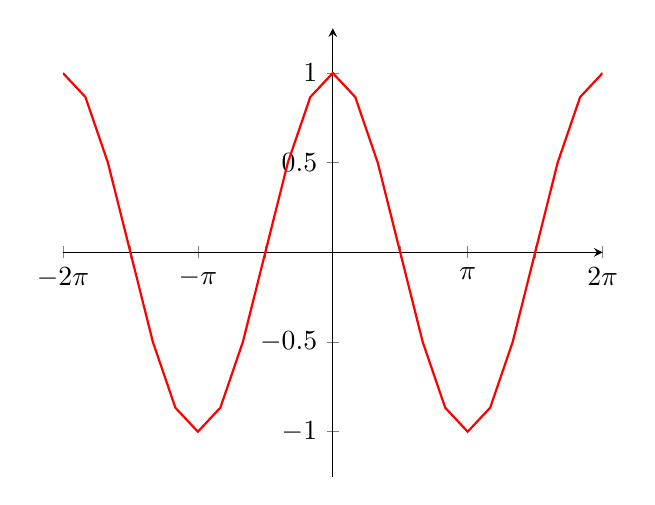
\begin{tikzpicture}
\begin{axis}[
    xmin=-2*pi,xmax=2*pi,
    ymin=-1.25,ymax=1.25,
    axis lines=middle,
	disabledatascaling,
    xtick={-2*pi, -(3/2)*pi, -pi, -(1/2)*pi, (1/2)*pi, pi, (3/2)*pi, 2*pi},
    xticklabels={$-2\pi$,,$-\pi$,,,$\pi$,,$2\pi$},
]

\addplot [samples=25,mark=none, thick, red,domain=-2*pi:2*pi] {cos(deg(x))};

\end{axis}
\end{tikzpicture}

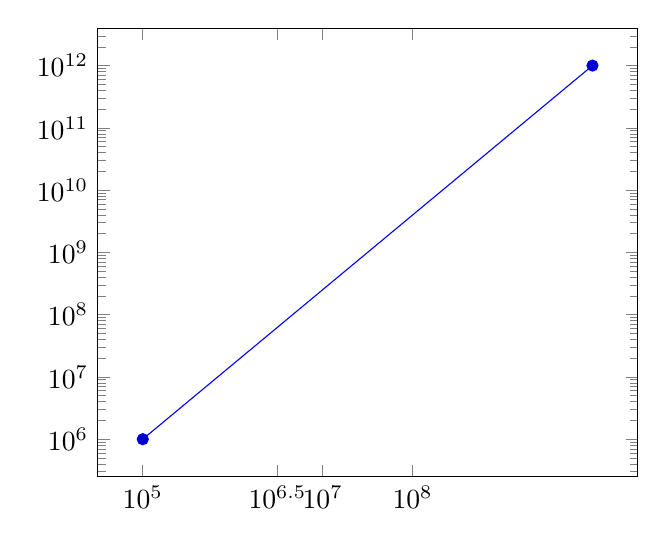
\begin{tikzpicture}
	\begin{loglogaxis}[
		xtick={1e5,pi*1e6,10*1e6,100*1e6},
	]
	\addplot coordinates {(1e5,1e6) (1e10,1e12)};
	\end{loglogaxis}
\end{tikzpicture}
\end{document}
